\documentclass[bachelor, och, coursework]{SCWorks}
% параметр - тип обучения - одно из значений:
%    spec     - специальность
%    bachelor - бакалавриат (по умолчанию)
%    master   - магистратура
% параметр - форма обучения - одно из значений:
%    och   - очное (по умолчанию)
%    zaoch - заочное
% параметр - тип работы - одно из значений:
%    referat    - реферат
%    coursework - курсовая работа (по умолчанию)
%    diploma    - дипломная работа
%    pract      - отчет по практике
%    pract      - отчет о научно-исследовательской работе
%    autoref    - автореферат выпускной работы
%    assignment - задание на выпускную квалификационную работу
%    review     - отзыв руководителя
%    critique   - рецензия на выпускную работу
% параметр - включение шрифта
%    times    - включение шрифта Times New Roman (если установлен)
%               по умолчанию выключен
\usepackage[T2A]{fontenc}
\usepackage[utf8x]{inputenc}
\usepackage{graphicx}

\usepackage[sort,compress]{cite}
\usepackage{amsmath}
\usepackage{amssymb}
\usepackage{amsthm}
\usepackage{fancyvrb}
\usepackage{longtable}
\usepackage{listings}
\usepackage{array}
\usepackage{float}
\usepackage[russian]{nomencl}
\usepackage[english,russian]{babel}

\usepackage[colorlinks=true]{hyperref}

\newcommand{\eqdef}{\stackrel {\rm def}{=}}
\newcommand{\No}{\textnumero}
\newtheorem{lem}{Лемма}

\lstset{
    breaklines=true, 
    language=Python, 
    numberstyle=\tiny, 
    numbers=left, 
    columns=flexible,
    keepspaces=false, 
    basicstyle=\small,
    tabsize=2,
    inputencoding=cp1251
}

\makeglossary
\renewcommand{\nomname}{Обозначения и сокращения}

\begin{document}

% Кафедра (в родительном падеже)
\chair{математической кибернетики и компьютерных наук}

% Тема работы
\title{Программно управляемые сети и их применение}

% Курс
\course{2}

% Группа
\group{251}

% Факультет (в родительном падеже) (по умолчанию "факультета КНиИТ")
%\department{факультета КНиИТ}

% Специальность/направление код - наименование
%\napravlenie{02.03.02 "--- Фундаментальная информатика и информационные технологии}
%\napravlenie{02.03.01 "--- Математическое обеспечение и администрирование информационных систем}
%\napravlenie{09.03.01 "--- Информатика и вычислительная техника}
\napravlenie{09.03.04 "--- Программная инженерия}
%\napravlenie{10.05.01 "--- Компьютерная безопасность}

% Для студентки. Для работы студента следующая команда не нужна.
%\studenttitle{Студентки}

% Фамилия, имя, отчество в родительном падеже
\author{Дергунова Дмитрия Витальевича}

% Заведующий кафедрой
\chtitle{к.\,ф.-м.\,н.} % степень, звание
\chname{С.\,В.\,Миронов}

%Научный руководитель (для реферата преподаватель проверяющий работу)
\satitle{доцент,\,к.\,т.\,н.} %должность, степень, звание
\saname{В.\,М.\,Соловьев}

% Руководитель практики от организации (только для практики,
% для остальных типов работ не используется)
%\patitle{Зав.\,каф.\,техн.\,прогр., к.\,ф.-м.\,н.}
%\paname{И.\,А.\,Батраева}

% Семестр (только для практики, для остальных
% типов работ не используется)
%\term{2}

% Наименование практики (только для практики, для остальных
% типов работ не используется)
%\practtype{учебная}

% Продолжительность практики (количество недель) (только для практики,
% для остальных типов работ не используется)
%\duration{2}

% Даты начала и окончания практики (только для практики, для остальных
% типов работ не используется)
%\practStart{30.06.2017}
%\practFinish{13.07.2017}

% Год выполнения отчета
\date{2018}

\maketitle

% Включение нумерации рисунков, формул и таблиц по разделам
% (по умолчанию - нумерация сквозная)
% (допускается оба вида нумерации)
%\secNumbering

% Путь к скриншотам
\graphicspath{{./images/}}

\tableofcontents

\printglossary

\intro
Управление компьютерными сетями, в основе которых лежит стек протоколов TCP/IP, является устаревшим и при передаче разнородного трафика имеет низкую эффективность. В современных сетях совмещены функции передачи данных и управления, что делает контроль и управление сетью очень сложными. Из-за сложности сетей затрудняется масштабирование и управление ими, снижается их надежность. Вследствие этого замедляется развитие сетей и приложений, работающих в них.
Новые разработки в области сетевых технологий, такие как программно-конфигурируемые сети (\nomenclature{ПКС}{Программно конфигурируемые сети}) и технология виртуализации сетевых функций (ВСФ) могут стать выходом из данной ситуации. Технология ВСФ необходима для решения проблем, связанных со временем развертывания компьютерных сетей и потреблением энергии сетевыми технологиями, так как текущая архитектура компьютерных сетей недостаточно энергоэффективна. \nomenclature{ПКС}{Программно конфигурируемые сети} позволяют упростить управление и администрирование сети, улучшить ее масштабируемость, увеличить пропускную способность каналов связи, автоматически перераспределять нагрузку на сетевые каналы и устройства. Благодаря этому центры обработки данных, владельцы компьютерных сетей, телекоммуникационные компании, интернет-провайдеры уменьшают затраты. При совокупном использовании этих двух технологий положительный эффект при построении компьютерных сетей будет наивысшим. Технология \nomenclature{ПКС}{Программно конфигурируемые сети} является базовой, в нее внедряется технология ВСФ.
Следует обратить внимание на недостатки нынешних компьютерных сетей, которые приводят к созданию технологии \nomenclature{ПКС}{Программно конфигурируемые сети}.
\begin{enumerate}
\item Высокая стоимость и сложность в обслуживании, так как они используют в своем строении сетевые устройства, которые сложны и реализуют все большее количество стандартов и протоколов. Это ведет к сбоям в работе систем, так как они не все имеют полное совмещение параметров. Обслуживающий персонал таких устройств должен быть высококвалифицированным.
\item В последнее время происходит значительный рост объема трафика. Большее число людей становится пользователями Интернета. Пропускная способность сетевых каналов связи компьютерных сетей истощается. Методы и средства контроля трафика не способны справиться с увеличивающейся каждый год нагрузкой.
\item В результате применения современными сетями закрытых и частных, запатентованных интерфейсов, появляются препятствия для разработки новых сервисов, нововведений и экспериментов.
\item В текущих сетевых технологиях используется набор сетевых протоколов, которые обеспечивают безопасную связь хостов в данной сети с использованием необходимой скорости соединения, учитывая конкретную сетевую топологию. Если обнаруживается новая проблема, то в стек протоколов TCP/IP дополняется новым протоколом, который решает данную проблему. Таким образом, количество стандартов и протоколов все время растет, в текущий момент времени количество протоколов преодолело отметку в 600 единиц.
\item В настоящее время производится увеличение облачных услуг, а пользователям необходимо увеличение скорости доступа к этим услугам.
\item Меняются модели передвижения трафика.
\end{enumerate}
Текущие возможности архитектуры компьютерных сетей не соответствуют требованиям рынка. Это привело к созданию архитектуры \nomenclature{ПКС}{Программно конфигурируемые сети}. \nomenclature{ПКС}{Программно конфигурируемые сети} – это сеть, которая функционирует отдельно от сетевых устройств, где программирование осуществляется напрямую. За счет этого сетевые сервисы и приложения отделяются от физического оборудования, и эта сеть рассматривается в виде виртуальной и логической сущности.
Задачи, которые преследуются при разработке технологии \nomenclature{ПКС}{Программно конфигурируемые сети}:
\begin{enumerate}
\item Цельное управление сетью;
\item Используя программное обеспечение, способное функционировать на отдельном компьютере и управляющееся сетевым администратором, отделить от функции передачи данных функцию управления сетевым оборудованием;
\item Между транспортной средой и сетевыми приложениями создать программно-управляемый интерфейс.
\nomenclature{ПКС}{Программно конфигурируемые сети} не является очередным механизмом улучшения работы сети и не является набором каких-либо новых протоколов для управления сетью. Создана новая архитектура сети, в которой абстрагирован уровень управления. Она использует уже имеющееся оборудование, принося качественные изменения в принципы его работы и организацию управления сетью.
\end{enumerate}


%----- Основная часть
\section{Теоретические сведения}\label{theory}
В архитектуру \nomenclature{ПКС}{Программно конфигурируемые сети} входят три уровня (смотри рисунок 1).
\begin{enumerate}
\item Уровень приложений, в который входит набор прикладных программ контроллера, необходимых для осуществления функций высокоэффективного управления сетью.
\item Уровень управления, в который входит сетевая операционная система (контроллер). С помощью нее осуществляется проверка состояния и работы сети и сетевых устройств. Эта операционная система предоставляет возможности находящемуся выше уровню для исполнения функций управления потоками данных в сети и сетевой инфраструктурой.
\item Уровень инфраструктуры включает в себя сетевые устройства и каналы передачи данных, которые образуют топологию сети.
\end{enumerate}
\begin{figure}[H]
    \centering
    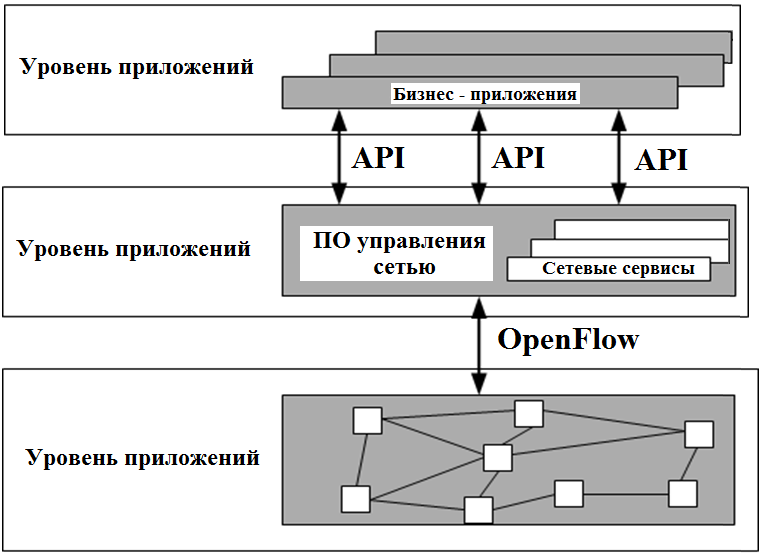
\includegraphics[width=\textwidth]{pic1}
    \caption{Архитектура \nomenclature{ПКС}{Программно конфигурируемые сети}}\label{fig:fact-02}
\end{figure}


% -------------------------------
% Раздел "Заключение"
\conclusion
В ходе курсовой работы *** 

% Список литературы
\bibliographystyle{gost780uv}
\bibliography{thesis}

% Окончание основного документа и начало приложений
% Каждая последующая секция документа будет являться приложением

\appendix
\section{USB-накопитель с отчетом о выполненной работе}\label{app:USB}
На приложенном USB-накопителe можно ознакомиться со следующими файлами:
\begin{description}
\item[Папка \texttt{tex}] "--- \LaTeX- вариант курсовой работы;
\item[\texttt{SoftwareDefinedNetworks.pdf}] "--- курсовая работа.
\end{description}

\end{document}
